\documentclass[journal,12pt,twocolumn]{IEEEtran}
\usepackage{graphicx}
\graphicspath{{./figs/}}{}
\usepackage{amsmath,amssymb,amsfonts,amsthm}
\newcommand{\myvec}[1]{\ensuremath{\begin{pmatrix}#1\end{pmatrix}}}
\providecommand{\norm}[1]{\lVert#1\rVert}
\usepackage{listings}
\usepackage{watermark}
\usepackage{titlesec}
\usepackage{caption}
\let\vec\mathbf
\lstset{
frame=single, 
breaklines=true,
columns=fullflexible
}
\thiswatermark{\centering \put(0,-105.0){
\includegraphics[scale=0.15]{/sdcard/IITH/vector/vectpr-4/figs/logo.png}} }
\title{\mytitle}
\title{
Assignment - Vector-4
}
\author{Surajit Sarkar}
\begin{document}
\maketitle
%\tableofcontents
\bigskip
\section{\textbf{Problem}}
Determine the ratio in which the line 2x+y–4=0 divides the line segment joining the points A(2,–2) and B(3,7).
\section{\textbf{Solution}}
\begin{table}[h]
    \centering
    \begin{tabular}{|c|c|}
       \hline
       \textbf{Symbol}&\textbf{Value}  \\
       \hline
	    $\vec{A}$ & $\myvec{2\\-2}$\\
        \hline
	    $\vec{B}$ & $\myvec{3\\7}$\\
        \hline
	    c&$4$\\
        \hline
       $\vec{n}$ & $\myvec{2\\1}$\\
       \hline
    \end{tabular}
    \caption{Parameters}
    \label{tab:my_label}
\end{table}
Given equation
\begin{align}
    \myvec{2&1}\vec{x}&=4\\
    \text{Using section formula}\\
    \text{Let the ratio be k:1}\\
    \vec{n}^{\top}\vec{P}&=c\\
    \implies\vec{n}^{\top}\myvec{\frac{k\vec{B+A}}{k+1}}&=c\\
    \implies\vec{n}^{\top}\myvec{k\vec{B+A}}&=c\myvec{k+1}\\
    \implies\vec{n}^{\top}k\vec{B}+\vec{n}^{\top}\vec{A}&=c\myvec{k+1}\\
    \implies k\vec{n}^{\top}\vec{B}+\vec{n}^{\top}\vec{A}&=c\myvec{k+1}\\
    \implies k\vec{n}^{\top}\vec{B}-ck&=-\vec{n}^{\top}\vec{A}+c\\
    \implies k\myvec{\vec{n}^{\top}\vec{B}-c}&=c-\vec{n}^{\top}\vec{A}\\
    \implies k&=\frac{c-\vec{n}^{\top}\vec{A}}{\vec{n}^{\top}\vec{B}-c}\\
    \implies k&=\frac{4-2}{13-4}\\
    \implies k&=\frac{2}{9}
\end{align}
\section{\textbf{Code Link}}
\begin{lstlisting}
https://github.com/sssurajit/fwc/blob/main/vector/vector-4/codes/vector.py
\end{lstlisting}
Execute the code by using the command\\
\textbf{python3 vector.py}
\section{\textbf{Figure}}
\begin{figure}[!h]
\centering
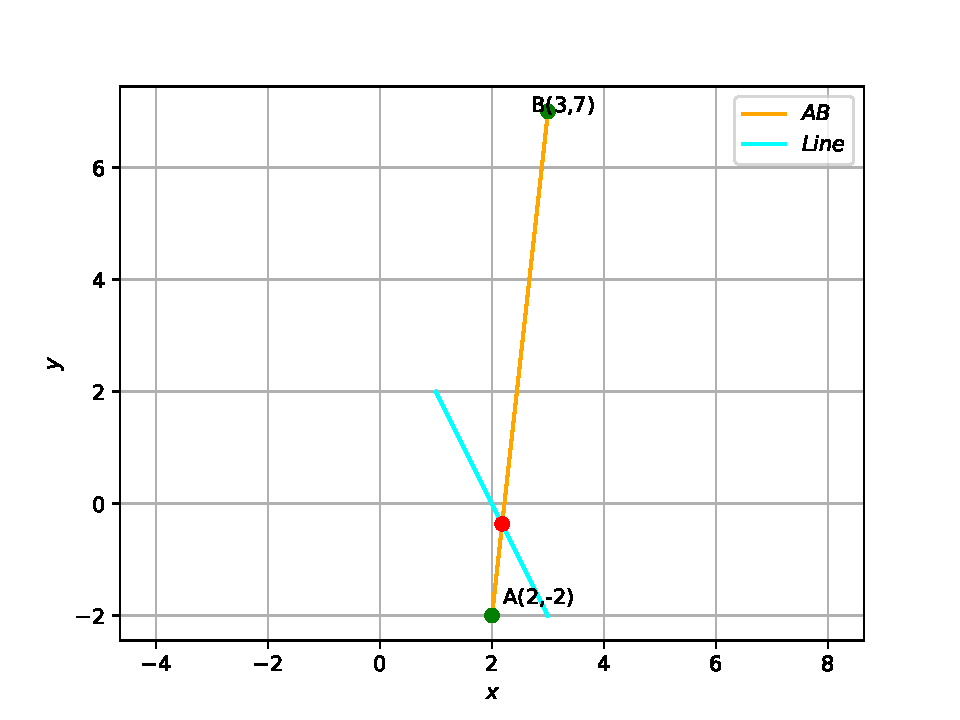
\includegraphics[width=\columnwidth]{/sdcard/IITH/vector/vectpr-4/figs/vec.pdf}
\caption{}
\label{fig:vec}
\end{figure}
\end{document}

